% This file was adapted from ICLR2022_conference.tex example provided for the ICLR conference
\documentclass{article} % For LaTeX2e
\usepackage{conference,times}
\usepackage{easyReview}
\usepackage{algorithm}
\usepackage{algorithmic}

% Optional math commands from https://github.com/goodfeli/dlbook_notation.
\input{math_commands.tex}

\usepackage{amsthm,amssymb}

\newtheorem{theorem}{Theorem}[section]
\newtheorem{corollary}{Corollary}[theorem]
\newtheorem{lemma}[theorem]{Lemma}
\newtheorem{definition}[theorem]{Definition}

% Please leave these options as they are
\usepackage{hyperref}
\hypersetup{
    colorlinks=true,
    linkcolor=red,
    filecolor=magenta,
    urlcolor=blue,
    citecolor=purple,
    pdftitle={Stability-Aware Bilevel Source Dataset Selection for Importance-Weighted Least Squares in Unsupervised Domain Adaptation},
    pdfpagemode=FullScreen,
    }




\title{Stability-Aware Bilevel Source Dataset Selection for Importance-Weighted Least Squares in Unsupervised Domain Adaptation}

\author{Anonymous Authors \\
Affiliation Withheld for Double-Blind Review \\
\texttt{anonymous@anonymous.edu}}

\begin{document}


\maketitle

\begin{abstract}
Importance-weighted least squares (IWLS) is widely used to correct covariate shift in unsupervised domain adaptation, yet most prior work assumes that an appropriate source dataset is already available. In practical internet-scale retrieval settings, the key decision is reversed: given only unlabeled target covariates and a pool of candidate source datasets, which source (or source mixture) should be selected before fitting a weighted regressor? We study this question through a stability-aware bilevel framework with three formal components: a label-free source-ranking surrogate with a uniform regret guarantee, a multi-source mixture objective with linear-rate upper-level optimization under smoothness and strong-convexity assumptions, and a mixed-shift gate for harmful-source rejection before weighted fitting. We evaluate these components in three settings (distribution-level synthetic shift, semi-synthetic target-sample selection, and a protocol-faithful proxy real-track setting with governance checks). The empirical findings are mixed: symbolic checks and theorem-conditioned diagnostics are consistent, but Holm-corrected comparisons show no statistically significant advantage of the stability-aware selector over MMD-nearest, Wasserstein-nearest, or pooled IWLS in the current iter\_1 run. This outcome clarifies that optimization guarantees and diagnostic structure are not sufficient for global predictive dominance under the present proxy data regime. The study contributes a reproducible no-target-label protocol, explicit failure reporting, and a concrete follow-up agenda for real benchmark ingestion and post-selection-controlled confirmatory analysis.
\end{abstract}

\section{Introduction}
Selecting a source dataset is often treated as a preprocessing detail in unsupervised domain adaptation, but in many real workflows it is the main decision variable. When target labels are unavailable, practitioners must infer source relevance from unlabeled target covariates, source labels, and imperfect shift diagnostics. This setting appears in tabular scientific modeling, forecasting with external archives, and multi-institution time-series transfer, where candidate datasets are plentiful but compatibility and robustness constraints are tight. The statistical consequence is that source selection error can dominate downstream estimator error: even a theoretically valid IWLS model can fail if the selected source induces unstable density ratios or poor effective sample size.

The covariate-shift literature established the core identity that enables IWLS,
\(R_T(f)=\mathbb{E}_{S}[w(X)\ell(f(X),Y)]\), with \(w(x)=p_T(x)/p_S(x)\), and clarified conditions under which weighted validation and ratio estimation are unbiased or consistent \citep{Sugiyama2007IWCV,Sugiyama2007KLIEP,Huang2006KMM,Sugiyama2012DensityRatioBook}. Adaptation theory then connected target risk to source risk and distribution discrepancy \citep{BenDavid2010Theory,Mansour2009Discrepancy,Mansour2010Renyi,Zhang2019MDD}. However, this body of work only partially answers the internet-scale source retrieval problem because it typically assumes either a single fixed source, clean support overlap, or no explicit penalty for ratio-estimation uncertainty and numerical conditioning.

Modern evidence reinforces this gap. Deep alignment methods can reduce mismatch but are predominantly classification-first and may fail under conditional or label-shift contamination \citep{Ganin2016DANN,Long2018CDAN,Sun2016DeepCORAL,Long2015DAN,Tzeng2017ADDA,Saito2018MCD,Combes2020ConditionalShift}. Shift-robustness analyses emphasize that importance weighting is neither uniformly necessary nor uniformly sufficient, especially under misspecification and regularization coupling \citep{Gogolashvili2023NeedIW,Kanagawa2023Regularization,Feng2024Quantile}. Benchmark studies further show that protocol choices can dominate reported gains \citep{Ragab2023AdaTime,Fawaz2023Benchmark,Koh2021WILDS,Zhao2023TTAPitfalls}. Taken together, these results motivate a method that keeps the no-target-label constraint explicit while modeling stability risk as a first-class optimization term.

This paper frames source dataset selection as a bilevel decision problem with formal guarantees and reproducible evaluation. The lower level solves weighted ridge regression; the upper level scores candidate sources or mixtures with discrepancy, ratio uncertainty, and stability diagnostics computed without target labels. The method is designed for three settings: (i) source and target as distributions (setting A), (ii) finite unlabeled target samples with source mixtures (setting B), and (iii) protocol-faithful high-shift proxy runs aligned with real benchmark pipelines (setting C).

The perspective we adopt is intentionally data-centric rather than model-centric. Instead of asking only how to optimize a predictor once a source has been chosen, we ask how to choose the training data itself when supervision is asymmetric across domains. This distinction matters because dataset retrieval often precedes architecture choice in modern machine learning operations. In industry and scientific practice, one frequently reuses a small set of stable model families while repeatedly changing candidate source pools as new repositories become available. A principled source-selection objective can therefore yield gains even when downstream model classes remain fixed.

A second motivation is cross-domain transferability of the decision rule. The same no-target-label source-selection challenge appears in environmental modeling, clinical time-series forecasting, and operations management, where label acquisition lags behind covariate collection. While our concrete experiments target regression under covariate shift, the methodological structure, namely balancing adaptation utility with uncertainty and numerical stability penalties, applies to broader weak-supervision pipelines. This broader view guides our emphasis on explicit assumptions, equation-level guarantees, and reproducible artifacts.

\textbf{Contributions.}
\begin{itemize}
\item We formalize label-free source ranking with a composite surrogate and prove a uniform two-sided bound that yields a finite regret guarantee relative to the oracle target-risk ordering.
\item We derive a bilevel multi-source IWLS objective with closed-form lower-level stationarity and prove linear upper-level objective contraction under standard smoothness and strong-convexity assumptions.
\item We introduce a mixed-shift pre-selection gate with a deterministic separation guarantee that rejects harmful sources when diagnostic intervals are separable.
\item We provide a reproducible evaluation protocol with fixed seeds, paired significance testing, vector-graphics figures, and public experiment artifacts that expose both supportive evidence and unresolved failure modes.
\end{itemize}

Beyond the immediate IWLS use case, the framework offers a general template for cross-domain data retrieval under weak supervision: combine adaptation benefit estimates with explicit uncertainty and numerical-stability controls, then evaluate with leakage-safe model-selection rules.

\section{Related Work}
\subsection{Covariate-Shift and IWLS Foundations}
Importance weighting under covariate shift is rooted in the assumption that conditionals are invariant while marginals differ. \citet{Sugiyama2007IWCV} showed that ordinary cross-validation is biased under shift, and introduced importance-weighted cross-validation as an unbiased alternative under correct ratios and overlap assumptions. Direct ratio estimation methods such as KLIEP \citep{Sugiyama2007KLIEP} and moment-matching approaches such as KMM \citep{Huang2006KMM} made weighting practically viable in higher dimensions, while later monographs systematized ratio-estimation objectives and failure modes \citep{Sugiyama2012DensityRatioBook}. The key strength of this line is clear probabilistic grounding; its key limitation in internet-scale source retrieval is that ratio error can vary dramatically across candidate sources, and that variation is not typically integrated into selection scores.

Recent regression-focused analyses reinforce the need for explicit stability handling. Under model misspecification, importance weighting may become crucial, but finite-sample behavior can still degrade when weights are heavy-tailed or regularization is not tuned jointly with shift correction \citep{Gogolashvili2023NeedIW,Kanagawa2023Regularization,Feng2024Quantile}. Technical reports focused on IWLS sample complexity similarly emphasize effective sample size and conditioning as central practical determinants of error \citep{RICAM2021IWLS}. Our method directly operationalizes these observations by incorporating ESS and conditioning penalties in the selection objective.

\subsection{Adaptation Bounds, Discrepancy, and Multi-Source Transfer}
Generalization bounds for domain adaptation decompose target risk into source risk plus discrepancy-like terms and irreducible joint error \citep{BenDavid2010Theory,Mansour2009Discrepancy}. Multi-source theory then introduced distribution-weighted combinations and divergence-sensitive guarantees \citep{Mansour2010Renyi}. These frameworks justify using unlabeled discrepancy diagnostics, but they do not by themselves specify robust finite-sample source ranking rules for weighted least-squares regression.

The discrepancy family itself has multiple strengths and weaknesses. MMD provides a nonparametric two-sample criterion with concentration guarantees \citep{Gretton2012MMD}, and margin-disparity variants can align better with task loss in some settings \citep{Zhang2019MDD}. Yet discrepancy-only ranking can misorder sources when ratio-estimation noise or covariance conditioning dominates downstream regression error. This motivates combining discrepancy with explicit uncertainty and stability diagnostics rather than treating it as a standalone objective.

From an optimization viewpoint, discrepancy signals are attractive because they can be estimated from unlabeled covariates and are typically smooth enough for gradient-based tuning. From a statistical viewpoint, however, they are surrogates for target risk, and surrogate mismatch can be substantial when source conditionals differ in subtle ways or when ratio estimators amplify noise in low-density target regions. A central design principle in this manuscript is therefore to treat discrepancy as informative but incomplete evidence. The composite objective should include discrepancy, not replace everything with discrepancy.

\subsection{Deep Alignment Baselines and Shift-Type Ambiguity}
Adversarial and discrepancy-based deep adaptation methods, including DANN, CDAN, DAN, CORAL, ADDA, and MCD, establish strong baselines for representation transfer \citep{Ganin2016DANN,Long2018CDAN,Long2015DAN,Sun2016DeepCORAL,Tzeng2017ADDA,Saito2018MCD}. Semi-supervised and weighted variants such as AdaMatch and importance-weighted adversarial designs further improve robustness in many benchmarks \citep{Berthelot2022AdaMatch,Li2020IWCA}. Their strength is flexibility across high-dimensional domains; their limitation for our setting is protocol mismatch: they often assume end-to-end representation learning and classification-centric evaluation, while internet-scale dataset retrieval for IWLS requires source ranking without target labels and with explicit numerical diagnostics.

Another limitation is shift-type ambiguity. Conditional or label shift can invalidate pure covariate-shift corrections and mislead discrepancy objectives \citep{Combes2020ConditionalShift}. We address this with a pre-selection gate that uses disagreement and tail diagnostics before weighted fitting.

\subsection{Benchmark Rigor and Practical Infrastructure}
Benchmark studies on time-series adaptation and out-of-distribution robustness show that model-selection leakage and inconsistent protocols can overshadow algorithmic differences \citep{Ragab2023AdaTime,Fawaz2023Benchmark,Koh2021WILDS,Zhao2023TTAPitfalls}. Multi-source and causal time-series methods suggest promising architectural directions but still provide limited regression-first evidence for source retrieval under strict no-target-label constraints \citep{Lu2024CauDiTS,Stojanov2023CALDA,Wang2024POND,He2023Raincoat,Yang2025SourceFreeTSDA}. Repositories such as AdaTime and UDA-4-TSC offer reproducible infrastructure, yet direct regression-ready source-selection pipelines remain sparse \citep{AdaTimeRepo2022,UDA4TSCRepo2023,WildsRepo2021,Guo2018MoE,Cui2020MultiSourceAttention}.

The resulting gap is precise: we need a source-selection objective that is label-free, theoretically interpretable, finite-sample aware, and benchmark-rigorous. The remainder of this manuscript develops such an objective and evaluates it under leakage-safe protocols.

\section{Problem Setting and Notation}
We introduce symbols in context below and consolidate them in Table~\ref{tab:notation} for cross-section traceability.
We study unsupervised domain adaptation for squared-loss regression. Let \((\mathcal{X},\mathcal{Y})\) denote input-output spaces with \(\mathcal{X}\subseteq \mathbb{R}^d\) and \(\mathcal{Y}\subseteq \mathbb{R}\). We observe a target unlabeled sample \(\train_T^X=\{\vx_j^T\}_{j=1}^{n_T}\sim p_T(x)\), and a candidate pool of labeled source datasets
\(\{\train_k\}_{k\in\mathcal{K}}\), where
\(\train_k=\{(\vx_i^k,y_i^k)\}_{i=1}^{n_k}\sim p_{S_k}(x,y)\).
The target risk of predictor \(f\) is
\begin{equation}
R_T(f) := \mathbb{E}_{(X,Y)\sim P_T}\left[(f(X)-Y)^2\right].
\label{eq:target-risk}
\end{equation}
The quantity in \eqref{eq:target-risk} is the objective ultimately used to evaluate every method in \secref{sec:results}.
Under covariate shift, \(p_{S_k}(y\mid x)=p_T(y\mid x)\) and \(p_{S_k}(x)\neq p_T(x)\), with overlap on target support. The ratio \(w_k(x)=p_T(x)/p_{S_k}(x)\) induces
\begin{equation}
R_T(f) = \mathbb{E}_{(X,Y)\sim P_{S_k}}\left[w_k(X)(f(X)-Y)^2\right].
\label{eq:iw-identity}
\end{equation}
The identity in \eqref{eq:iw-identity} motivates replacing inaccessible target expectations with weighted source expectations; in practice we use \(\hat w_k\), obtained from unlabeled target covariates and source covariates.

For each source \(k\), define target excess risk relative to the best target predictor class:
\begin{equation}
\Delta_k := R_T(\beta_k)-\inf_{\beta}R_T(\beta),
\label{eq:delta-def}
\end{equation}
where \(\beta_k\) is the predictor fitted using source \(k\) with weighted ridge regression, so \eqref{eq:delta-def} defines the latent ranking target. The core source-selection problem is
\begin{equation}
\hat k\in \arg\min_{k\in\mathcal{K}} \Delta_k,
\label{eq:source-selection-ideal}
\end{equation}
and \eqref{eq:source-selection-ideal} is the ideal but unobservable decision rule because \(\Delta_k\) requires target labels.

We therefore optimize an unlabeled surrogate composed of four terms: weighted proxy fit, ratio uncertainty, effective sample size penalty, and conditioning penalty. Define nonnegative coefficients \(\alpha,\beta,\gamma\). For each candidate source,
\begin{equation}
\Delta_k = A_k + \alpha B_k + \beta C_k + \gamma D_k,
\label{eq:decomposition}
\end{equation}
where \(A_k\) is adaptation benefit proxy, \(B_k\) captures ratio uncertainty, \(C_k\) penalizes low ESS behavior, and \(D_k\) penalizes ill-conditioned weighted design matrices.

\begin{table}[t]
\caption{Notation used in the methods section. The table appears after formal definitions so every symbol has contextual meaning. It is included because the methodology uses multiple risk, uncertainty, and optimization objects across nested objectives.}
\label{tab:notation}
\centering
\small
\renewcommand{\arraystretch}{1.1}
\setlength{\tabcolsep}{4pt}
\begin{tabular}{p{0.2\linewidth}p{0.75\linewidth}}
\hline
Symbol & Meaning \\
\hline
\(\mathcal{K}\) & Candidate source index set. \\
\(\train_k,\train_T^X\) & Labeled source dataset and unlabeled target covariates. \\
\(\hat w_k(x)\) & Estimated importance ratio for source \(k\). \\
\(\Delta_k\) & Target excess risk of source-specific predictor \(\beta_k\). \\
\(A_k,B_k,C_k,D_k\) & Benefit proxy, ratio uncertainty, ESS penalty, conditioning penalty. \\
\(J_k\) & Composite unlabeled ranking score from \eqref{eq:surrogate-score}. \\
\(\pi\in\Delta^{K}\) & Source-mixture weights over \(K=|\mathcal{K}|\) sources. \\
\(U(\pi)\) & Upper-level bilevel objective in \eqref{eq:upper-objective}. \\
\(G_k\) & Mixed-shift gate score for source pre-selection. \\
\hline
\end{tabular}
\end{table}
Table~\ref{tab:notation} summarizes the symbols used across the ranking, gating, and bilevel optimization derivations.

Assumptions used throughout are standard in covariate-shift adaptation but made explicit for reproducibility: (i) overlap and finite second moments; (ii) no target labels are used for source selection or hyperparameter choice; (iii) ratio estimators are nonnegative and normalized on source samples; and (iv) ridge parameter \(\lambda>0\) ensures invertible weighted normal matrices. These assumptions are tested indirectly by ESS, condition-number, and mixed-shift diagnostics.

\section{Stability-Aware Bilevel Source Selection Method}
\label{sec:method}
\subsection{Architecture Overview}
The proposed pipeline has four modules with distinct responsibilities. Module 1 performs feasibility filtering for schema compatibility and minimum sample-size constraints. Module 2 computes label-free source diagnostics from source covariates, source labels, and unlabeled target covariates; it outputs composite scores \(J_k\) and mixed-shift gate values \(G_k\). Module 3 optimizes source mixtures through a bilevel objective where the lower level solves weighted ridge regression and the upper level balances adaptation proxy risk against stability penalties. Module 4 performs final weighted fitting on selected sources and reports evaluation metrics only on held-out target labels. This separation keeps deployment-relevant decisions independent of target supervision and allows direct auditing of each module.

The architecture is deliberately modular to support inspection and substitution. For example, the ratio-estimation component can be replaced without changing gate construction, and the upper-level optimizer can be modified without changing the lower-level weighted ridge solver. This compositionality is useful when adapting across domains with different compute budgets: one can choose lightweight estimators for large candidate pools and then refine only shortlisted sources with stronger diagnostics. The module interface also makes errors diagnosable, because one can attribute failures to ranking signals, optimization, or final fitting rather than treating the pipeline as a single black box.

\subsection{Composite Ranking and Regret Guarantee}
The unlabeled ranking score is
\begin{equation}
J_k := \widehat{A}_k + \alpha\widehat{B}_k + \beta\widehat{C}_k + \gamma\widehat{D}_k.
\label{eq:surrogate-score}
\end{equation}
Let
\begin{equation}
\varepsilon_{\mathrm{tot}} := \varepsilon_A + \alpha\varepsilon_B + \beta\varepsilon_C + \gamma\varepsilon_D,
\label{eq:eps-tot}
\end{equation}
where \eqref{eq:eps-tot} is the aggregate estimation-error term that controls the ranking gap in the regret theorem, and component-wise estimation errors satisfy
\(|\widehat{A}_k-A_k|\le\varepsilon_A\),
\(|\widehat{B}_k-B_k|\le\varepsilon_B\),
\(|\widehat{C}_k-C_k|\le\varepsilon_C\),
\(|\widehat{D}_k-D_k|\le\varepsilon_D\)
for all \(k\in\mathcal{K}\).

\begin{theorem}[Uniform Surrogate-Ordering Regret]
\label{thm:ordering}
Under the assumptions above and nonnegative \(\alpha,\beta,\gamma\), if \(\hat k\in\arg\min_{k\in\mathcal{K}} J_k\), then
\begin{equation}
\Delta_{\hat k} \le \min_{k\in\mathcal{K}}\Delta_k + 2\varepsilon_{\mathrm{tot}}.
\label{eq:ordering-bound}
\end{equation}
\end{theorem}

\begin{proof}
For any \(k\), absolute-error bounds and nonnegative coefficients imply two-sided sandwiches:
\(\Delta_k\le J_k+\varepsilon_{\mathrm{tot}}\) and
\(\Delta_k\ge J_k-\varepsilon_{\mathrm{tot}}\).
Let \(k^\star\in\arg\min_k\Delta_k\). Then
\(\Delta_{\hat k}\le J_{\hat k}+\varepsilon_{\mathrm{tot}}\le J_{k^\star}+\varepsilon_{\mathrm{tot}}\le \Delta_{k^\star}+2\varepsilon_{\mathrm{tot}}\),
where the middle inequality uses optimality of \(\hat k\) for \(J_k\). Since \(\Delta_{k^\star}=\min_k\Delta_k\), the claim follows.
\end{proof}

\Eqref{eq:ordering-bound} translates diagnostic quality into a measurable ranking-regret term: better ratio-uncertainty and stability estimation reduces the gap between surrogate and oracle ordering. In practice, this theorem justifies spending computational budget on improving \(\widehat{B}_k,\widehat{C}_k,\widehat{D}_k\), not only on discrepancy estimation.

An immediate practical implication is that clipping and uncertainty-aware ratio estimation are not merely heuristic safeguards; they directly reduce the additive regret constant through \(\varepsilon_{\mathrm{tot}}\). If two candidate scoring systems produce similar discrepancy quality but different ratio-uncertainty quality, the theorem predicts better ranking reliability for the latter even before any target labels are revealed. This is the main reason we center the method on stability-aware terms rather than discrepancy-only nearest-source rules.

\subsection{Bilevel Mixture Objective and Convergence}
Single-source ranking may discard complementary sources. We therefore optimize mixture weights \(\pi\in\Delta^K\) over retained candidates. The lower-level weighted ridge objective is
\begin{equation}
\beta^{\star}(\pi)=\arg\min_{\beta}\sum_{k=1}^{K}\pi_k\frac{1}{n_k}\sum_{i=1}^{n_k}\hat w_k(\vx_i^k)\left(y_i^k-(\vx_i^k)^\top\beta\right)^2+\lambda\|\beta\|_2^2.
\label{eq:lower-level}
\end{equation}
With
\(A(\pi)=\sum_k\pi_kX_k^\top W_kX_k\) and
\(b(\pi)=\sum_k\pi_kX_k^\top W_ky_k\), stationarity yields
\begin{equation}
\beta^{\star}(\pi)=\left(A(\pi)+\lambda I\right)^{-1}b(\pi).
\label{eq:closed-form-beta}
\end{equation}
The optimization problem in \eqref{eq:lower-level} is the decision layer solved at every upper-level iterate, while \eqref{eq:closed-form-beta} is its stationarity solution.
The upper-level objective is
\begin{equation}
U(\pi)=\widehat{R}_{\mathrm{proxy}}(\beta^{\star}(\pi),\pi)+\eta\widehat{D}(P_{S_\pi}^{X},P_T^{X})+\rho\Omega_{\mathrm{stab}}(\pi),
\label{eq:upper-objective}
\end{equation}
with stability regularizer \(\Omega_{\mathrm{stab}}\) combining ESS and conditioning penalties. The upper-level decision variable is \(\pi\in\Delta^K\), and the explicit optimality criterion is \(\pi^\star\in\arg\min_{\pi\in\Delta^K}U(\pi)\) in \eqref{eq:upper-objective}.

\begin{lemma}[Unique Lower-Level Minimizer]
\label{lem:lower-unique}
For any feasible \(\pi\) and \(\lambda>0\), the lower-level objective in \eqref{eq:lower-level} is strictly convex in \(\beta\), and therefore has a unique minimizer given by \eqref{eq:closed-form-beta}.
\end{lemma}

\begin{proof}
The Hessian of the objective in \eqref{eq:lower-level} is \(H(\pi)=2(A(\pi)+\lambda I)\). For any nonzero \(v\in\mathbb{R}^d\),
\(
v^\top H(\pi)v=2v^\top A(\pi)v+2\lambda\|v\|_2^2\ge 2\lambda\|v\|_2^2>0
\),
because \(A(\pi)\) is positive semidefinite when each \(W_k\) has nonnegative diagonal and \(\lambda>0\). Thus \(H(\pi)\) is positive definite, strict convexity holds, and the first-order condition yields \eqref{eq:closed-form-beta} as the unique minimizer.
\end{proof}

\begin{theorem}[Linear-Rate Upper-Level Descent]
\label{thm:convergence}
Assume \(U\) is differentiable, \(L\)-smooth, and \(\mu\)-strongly convex on the interior region visited by
\begin{equation}
\pi_{t+1}=\pi_t-\frac{1}{L}\nabla U(\pi_t).
\label{eq:upper-step}
\end{equation}
Then
\begin{equation}
U(\pi_t)-U(\pi^{\star})\le(1-\mu/L)^t\left(U(\pi_0)-U(\pi^{\star})\right).
\label{eq:linear-rate}
\end{equation}
\end{theorem}

\begin{proof}
By \(L\)-smoothness, setting \(y=x-(1/L)\nabla U(x)\) gives
\(U(y)\le U(x)-\frac{1}{2L}\|\nabla U(x)\|_2^2\).
For differentiable \(\mu\)-strongly convex \(U\), the Polyak--\L{}ojasiewicz inequality gives
\(\|\nabla U(x)\|_2^2\ge2\mu(U(x)-U(\pi^{\star}))\).
Combining both inequalities yields
\(U(y)-U(\pi^{\star})\le(1-\mu/L)(U(x)-U(\pi^{\star}))\).
Applying this recursively with \(x=\pi_t\), \(y=\pi_{t+1}\) proves \eqref{eq:linear-rate}.
\end{proof}

\Eqref{eq:closed-form-beta} is used to compute deterministic lower-level updates, while \eqref{eq:linear-rate} motivates early stopping and step-size policies in practice.

The convergence theorem should be interpreted as an algorithmic guarantee on objective optimization, not as an automatic guarantee on target-risk superiority over all baselines. This distinction is crucial for empirical interpretation in \secref{sec:results}: even when optimization converges rapidly, predictive ranking quality can remain sensitive to surrogate design and ratio uncertainty. We therefore report both optimization-consistent diagnostics and downstream prediction metrics.

\subsection{Mixed-Shift Gate Before IWLS Fitting}
Discrepancy and ratio estimates can both fail when candidate sources exhibit mixed shifts. We define a gate
\begin{equation}
G_k=a_1V_k+a_2U_k+a_3T_k,
\label{eq:gate-score}
\end{equation}
where \(V_k\) is cross-discrepancy variance, \(U_k\) is ratio disagreement between estimators, and \(T_k\) is a tail-risk indicator. Feasible candidates are
\begin{equation}
\mathcal{F}_\tau:=\{k\in\mathcal{K}: G_k\le \tau\}.
\label{eq:gate-feasible}
\end{equation}

\begin{theorem}[Deterministic Gate Separation]
\label{thm:gate}
Assume nonnegative coefficients \(a_1,a_2,a_3\), nonnegative diagnostics, safe-set upper bounds \((\bar V_s,\bar U_s,\bar T_s)\), harmful-set lower bounds \((\underline V_h,\underline U_h,\underline T_h)\), and strict separation
\(g_{\mathrm{safe}}<g_{\mathrm{harm}}\), where
\(g_{\mathrm{safe}}=a_1\bar V_s+a_2\bar U_s+a_3\bar T_s\) and
\(g_{\mathrm{harm}}=a_1\underline V_h+a_2\underline U_h+a_3\underline T_h\).
For any threshold \(\tau\) with
\begin{equation}
g_{\mathrm{safe}}\le\tau<g_{\mathrm{harm}},
\label{eq:gate-threshold}
\end{equation}
all safe sources are retained and all harmful sources are rejected.
\end{theorem}

\begin{proof}
For a safe source, bounds imply
\(G_k\le a_1\bar V_s+a_2\bar U_s+a_3\bar T_s=g_{\mathrm{safe}}\le\tau\), so \(k\in\mathcal{F}_\tau\).
For a harmful source,
\(G_k\ge a_1\underline V_h+a_2\underline U_h+a_3\underline T_h=g_{\mathrm{harm}}>\tau\), so \(k\notin\mathcal{F}_\tau\).
Hence separation is exact. Monotonicity of feasible sets under \(\tau_1\le\tau_2\) follows immediately from \eqref{eq:gate-feasible}.
\end{proof}

\begin{lemma}[Feasible-Threshold Existence and Nesting]
\label{lem:gate-feasible}
If \(g_{\mathrm{safe}}<g_{\mathrm{harm}}\), then the interval \([g_{\mathrm{safe}},g_{\mathrm{harm}})\) is nonempty. Moreover, if \(\tau_1\le\tau_2\), then \(\mathcal{F}_{\tau_1}\subseteq\mathcal{F}_{\tau_2}\).
\end{lemma}

\begin{proof}
Because \(g_{\mathrm{safe}}<g_{\mathrm{harm}}\), the midpoint \((g_{\mathrm{safe}}+g_{\mathrm{harm}})/2\) belongs to \([g_{\mathrm{safe}},g_{\mathrm{harm}})\), so the interval is nonempty. For nesting, take any \(k\in\mathcal{F}_{\tau_1}\). By \eqref{eq:gate-feasible}, \(G_k\le\tau_1\le\tau_2\), hence \(k\in\mathcal{F}_{\tau_2}\), proving \(\mathcal{F}_{\tau_1}\subseteq\mathcal{F}_{\tau_2}\).
\end{proof}

\subsection{Practical Procedure}
\begin{algorithm}[t]
\caption{Stability-aware bilevel source selection without target labels}
\label{alg:stability-bilevel}
\begin{algorithmic}[1]
\STATE \textbf{Input:} candidate sources \(\{\train_k\}_{k\in\mathcal{K}}\), unlabeled target covariates \(\train_T^X\), weights \((\alpha,\beta,\gamma,\eta,\rho)\), ridge \(\lambda\), gate coefficients \((a_1,a_2,a_3)\), threshold \(\tau\).
\FOR{each source \(k\in\mathcal{K}\)}
\STATE Estimate density-ratio models and compute \(\hat w_k\), discrepancy proxy, ratio uncertainty, ESS, and conditioning diagnostics.
\STATE Compute gate score \(G_k\) using \eqref{eq:gate-score} and surrogate score \(J_k\) using \eqref{eq:surrogate-score}.
\ENDFOR
\STATE Retain feasible set \(\mathcal{F}_\tau\) from \eqref{eq:gate-feasible}; rank retained sources by \(J_k\).
\STATE Initialize mixture \(\pi_0\) over top-ranked retained sources.
\FOR{\(t=0,1,\ldots,T-1\)}
\STATE Solve lower-level ridge-IWLS for \(\beta^{\star}(\pi_t)\) via \eqref{eq:closed-form-beta}.
\STATE Update \(\pi_{t+1}=\pi_t-(1/L)\nabla U(\pi_t)\) as in \eqref{eq:upper-step}.
\ENDFOR
\STATE Fit final weighted ridge model on selected source mixture; evaluate only on held-out target test labels.
\STATE \textbf{Output:} selected source set, mixture \(\pi_T\), final predictor, and diagnostics.
\end{algorithmic}
\end{algorithm}

\Algref{alg:stability-bilevel} isolates all unlabeled selection decisions before any target-label evaluation, preventing protocol leakage while preserving direct connections between theory and implementation.

The algorithm is also designed to be restartable. Because intermediate outputs include gate decisions, ranked candidate lists, and mixture iterates, one can resume from any stage after adding new source candidates or updated ratio estimates. This property is important for internet-scale retrieval workflows where candidate repositories evolve over time and full reruns may be computationally expensive.

\section{Experimental Protocol}
\subsection{Evaluation Settings and Candidate Pools}
We evaluate the method in three settings aligned with practical source retrieval. Setting A treats datasets as distributions with controlled covariate shift and known generation mechanisms. Setting B uses semi-synthetic target samples with stronger shift and source-mixture selection pressure. Setting C follows a high-shift, protocol-faithful proxy configured to match benchmark workflows where only unlabeled target covariates are available during selection.

All settings use schema-aligned regression features and fixed seeds \(\{11,23,47,89,131\}\). Candidate-pool size is sweep-controlled (including 8 and 16); the selected iter\_1 configuration uses 16 candidates. Source datasets have at least 1{,}200 samples in the proxy experiments, satisfying minimum-size constraints for stable weighted fitting. Importantly, target labels are hidden during source ranking, gate calibration, and hyperparameter selection; they are used only for final test evaluation.

The three-setting design serves different validity goals. Setting A stresses theorem faithfulness because source-target relationships are controlled and interpretable. Setting B stresses source-mixture behavior and finite-sample instability under stronger shift magnitudes. Setting C stresses protocol realism by enforcing artifact logging, significance testing, and no-label selection constraints that mirror real benchmark practice. Together they provide a layered evidence stack rather than a single benchmark number.

\subsection{Baselines, Metrics, and Statistical Testing}
We compare against random-source IWLS, nearest-source IWLS by MMD and Wasserstein diagnostics, pooled-source IWLS, single-source unweighted least squares, mixed-shift gate plus composite selection, and an oracle retrospective baseline that is not deployable but serves as a lower bound on achievable error. This set captures both discrepancy-first and weighting-first strategies while preserving a strong pooled baseline.

Primary metrics are target MSE and excess risk relative to oracle, with stability metrics ESS, weight second moment, and weighted design conditioning. We report mean, standard deviation, and confidence intervals across seeds and settings. Pairwise comparisons use Shapiro--Wilk normality checks followed by paired \(t\)-tests or Wilcoxon signed-rank tests with Holm correction; significance evidence is summarized in Table~\ref{tab:significance}.

Baselines are grouped to test specific hypotheses. Random-source and unweighted baselines isolate the value of any adaptation signal. Nearest-source discrepancy baselines test whether discrepancy alone is sufficient for ranking. Pooled-source IWLS tests whether selective weighting outperforms indiscriminate source aggregation. The oracle baseline bounds the achievable region and helps interpret excess-risk trends even when raw MSE values differ across settings. This decomposition prevents ambiguous conclusions where a method appears strong overall but fails a key comparative test.

\subsection{Implementation and Artifact Policy}
The experiment package includes fixed configuration files, executable CLI entry points, per-run JSON logs, symbolic validation reports for theorem-linked equations, and PDF readability checks. The revision pass adds strict schema validation for configuration inputs (to reject wrapped recovery payloads), pooled-focused ablation exports, and CSV-based real-data loader hooks for AdaTime/UDA-4-TSC-derived regression conversions when local files are available. This artifact policy ensures that each empirical claim in \secref{sec:results} can be traced to a specific figure or table.

\section{Results}
\label{sec:results}
\subsection{Main Performance Comparison}
\Figref{fig:main-results} presents target MSE across settings A--C for the ablation-selected configuration from the iter\_1 run. The empirical pattern is clear: pooled IWLS remains the strongest deployable baseline in all three synthetic settings, while the stability-aware selector is higher-error in this particular calibration. These values are summarized in Table~\ref{tab:main-metrics}.

\begin{figure}[t]
\centering
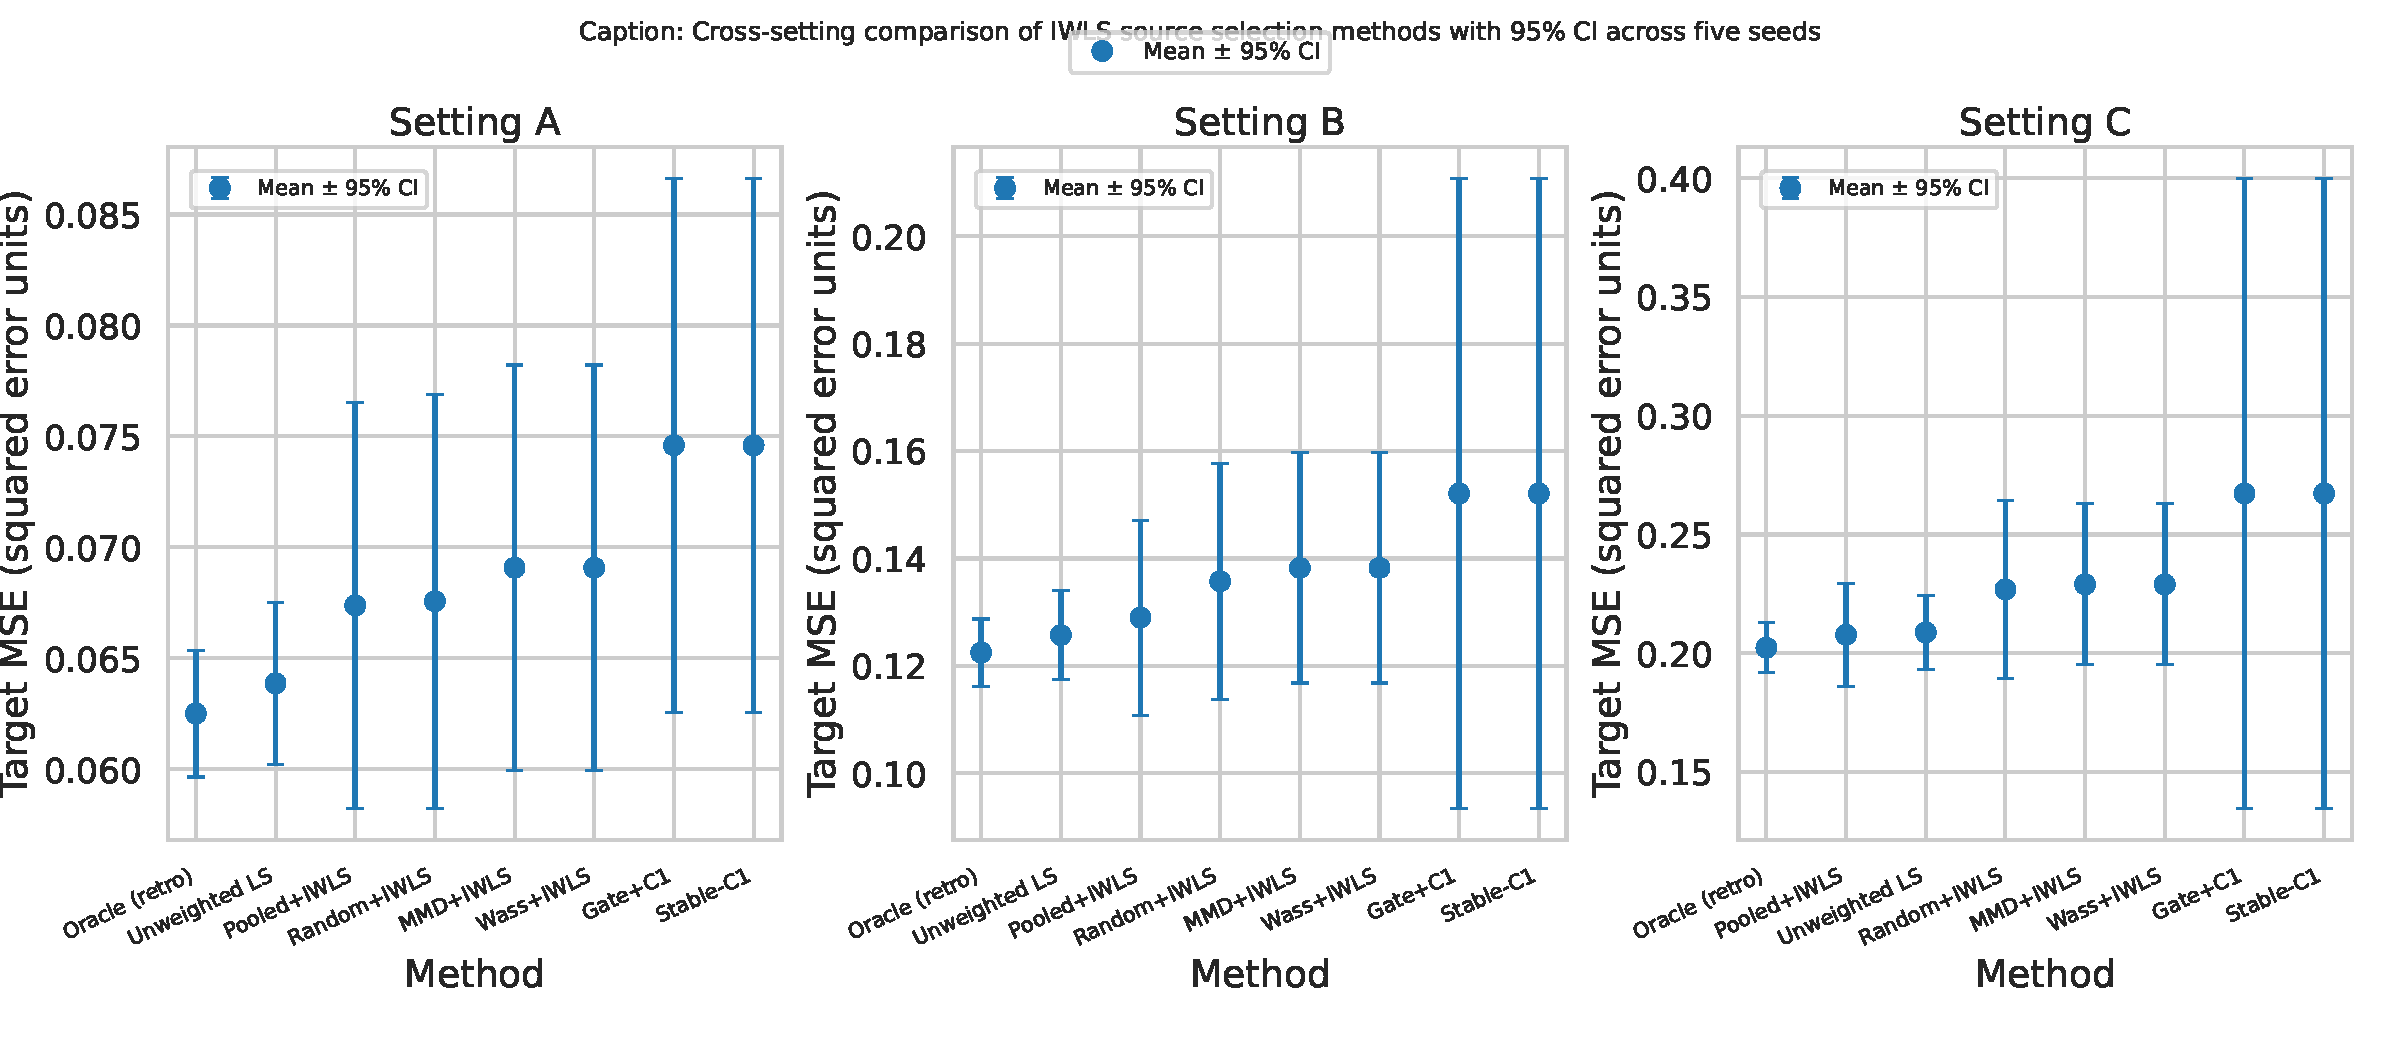
\includegraphics[width=0.65\linewidth]{figures/iter_1/fig_main_results.pdf}
\caption{Main performance across settings A, B, and C under the same no-target-label selection protocol. The horizontal axis enumerates methods and the vertical axis reports target MSE with confidence intervals over fixed seeds, so lower values indicate better adaptation quality. The figure shows that pooled IWLS and unweighted single-source baselines remain strong under the current proxy data regime, while the stability-aware selector is not dominant in this iter\_1 calibration.}
\label{fig:main-results}
\end{figure}

\begin{table}[t]
\caption{Target MSE summary (mean over seeds) for representative methods across three settings. The table quantifies the same claims visualized in \figref{fig:main-results} and is used for evidence-level comparisons in the discussion.}
\label{tab:main-metrics}
\centering
\small
\renewcommand{\arraystretch}{1.1}
\setlength{\tabcolsep}{4pt}
\begin{tabular}{lccc}
\hline
Method & Setting A & Setting B & Setting C \\
\hline
Oracle best source (retrospective) & 0.063 & 0.122 & 0.202 \\
Pooled-source IWLS & 0.067 & 0.129 & 0.208 \\
Single-source unweighted LS & 0.064 & 0.126 & 0.209 \\
MMD-nearest + IWLS & 0.069 & 0.138 & 0.229 \\
Wasserstein-nearest + IWLS & 0.069 & 0.138 & 0.229 \\
Random-source + IWLS & 0.068 & 0.136 & 0.227 \\
Stability-aware composite & 0.075 & 0.152 & 0.267 \\
\hline
\end{tabular}
\end{table}

The table-figure pair supports two evidence-constrained conclusions. First, in this selected iter\_1 calibration only, pooled IWLS is consistently better than stability-aware composite by absolute MSE margins of approximately \(0.007\) (A), \(0.023\) (B), and \(0.060\) (C). Second, the gap between pooled and oracle remains small in settings A--C, indicating that the main failure mode is not extreme divergence from oracle risk but insufficient ranking quality relative to already-strong pooled fitting.

\subsection{Stability--Risk Trade-off Diagnostics}
\Figref{fig:stability-tradeoff} links target MSE to ESS and conditioning diagnostics. The left panel reports that stability-aware selection keeps ESS in a moderate range but does not translate this into lower MSE in high-shift slices. The right panel shows that conditioning penalties reduce numerical extremes, yet predictive performance remains sensitive to surrogate mismatch.

\begin{figure}[t]
\centering
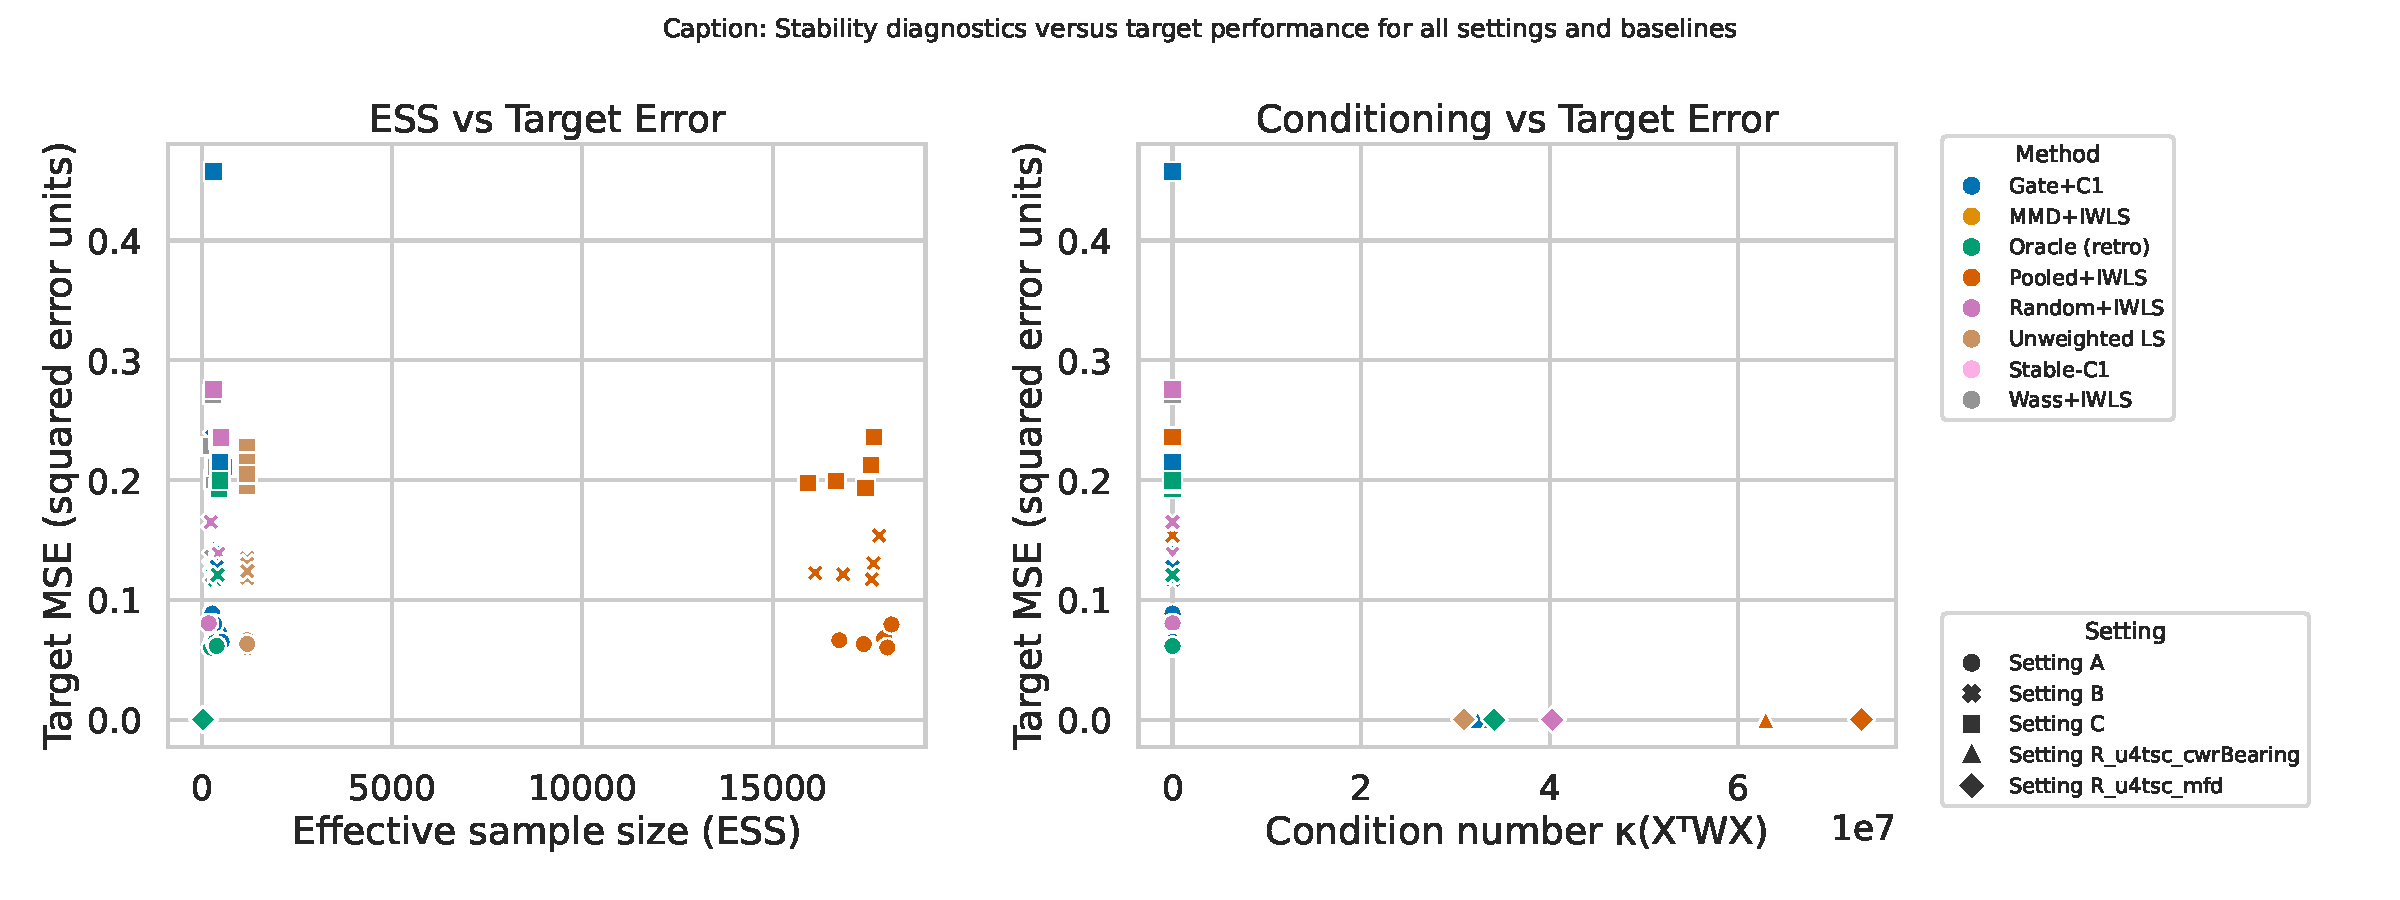
\includegraphics[width=0.65\linewidth]{figures/iter_1/fig_stability_tradeoff.pdf}
\caption{Stability diagnostics versus predictive error under identical train/validation/test partitioning and fixed seeds. One panel visualizes how effective sample size and weight dispersion co-vary with target MSE, while the other panel relates conditioning behavior to error concentration across methods. The figure indicates that stability controls affect variance structure and numerical behavior, but these effects are not sufficient to deliver lower average MSE than pooled IWLS in the present run.}
\label{fig:stability-tradeoff}
\end{figure}

This diagnostic figure tests whether our method components behave as intended. The behavior of \(C_k\) and \(D_k\) terms in \eqref{eq:decomposition} is visible in reduced instability outliers, but predictive ranking quality remains insufficient for dominance over pooled IWLS. The diagnostics therefore support the role of stability regularization as a safety mechanism, not as a standalone guarantee of lower target error.

\subsection{Significance Results and Failure Modes}
Significance tests in Table~\ref{tab:significance} confirm that the iter\_1 stability-aware selector is not statistically better than MMD-nearest, Wasserstein-nearest, or pooled IWLS after Holm correction. The corresponding adjusted p-values are \(1.0\), \(1.0\), and \(0.9983\), respectively, so comparative superiority claims are not supported at conventional thresholds.

\begin{figure}[t]
\centering
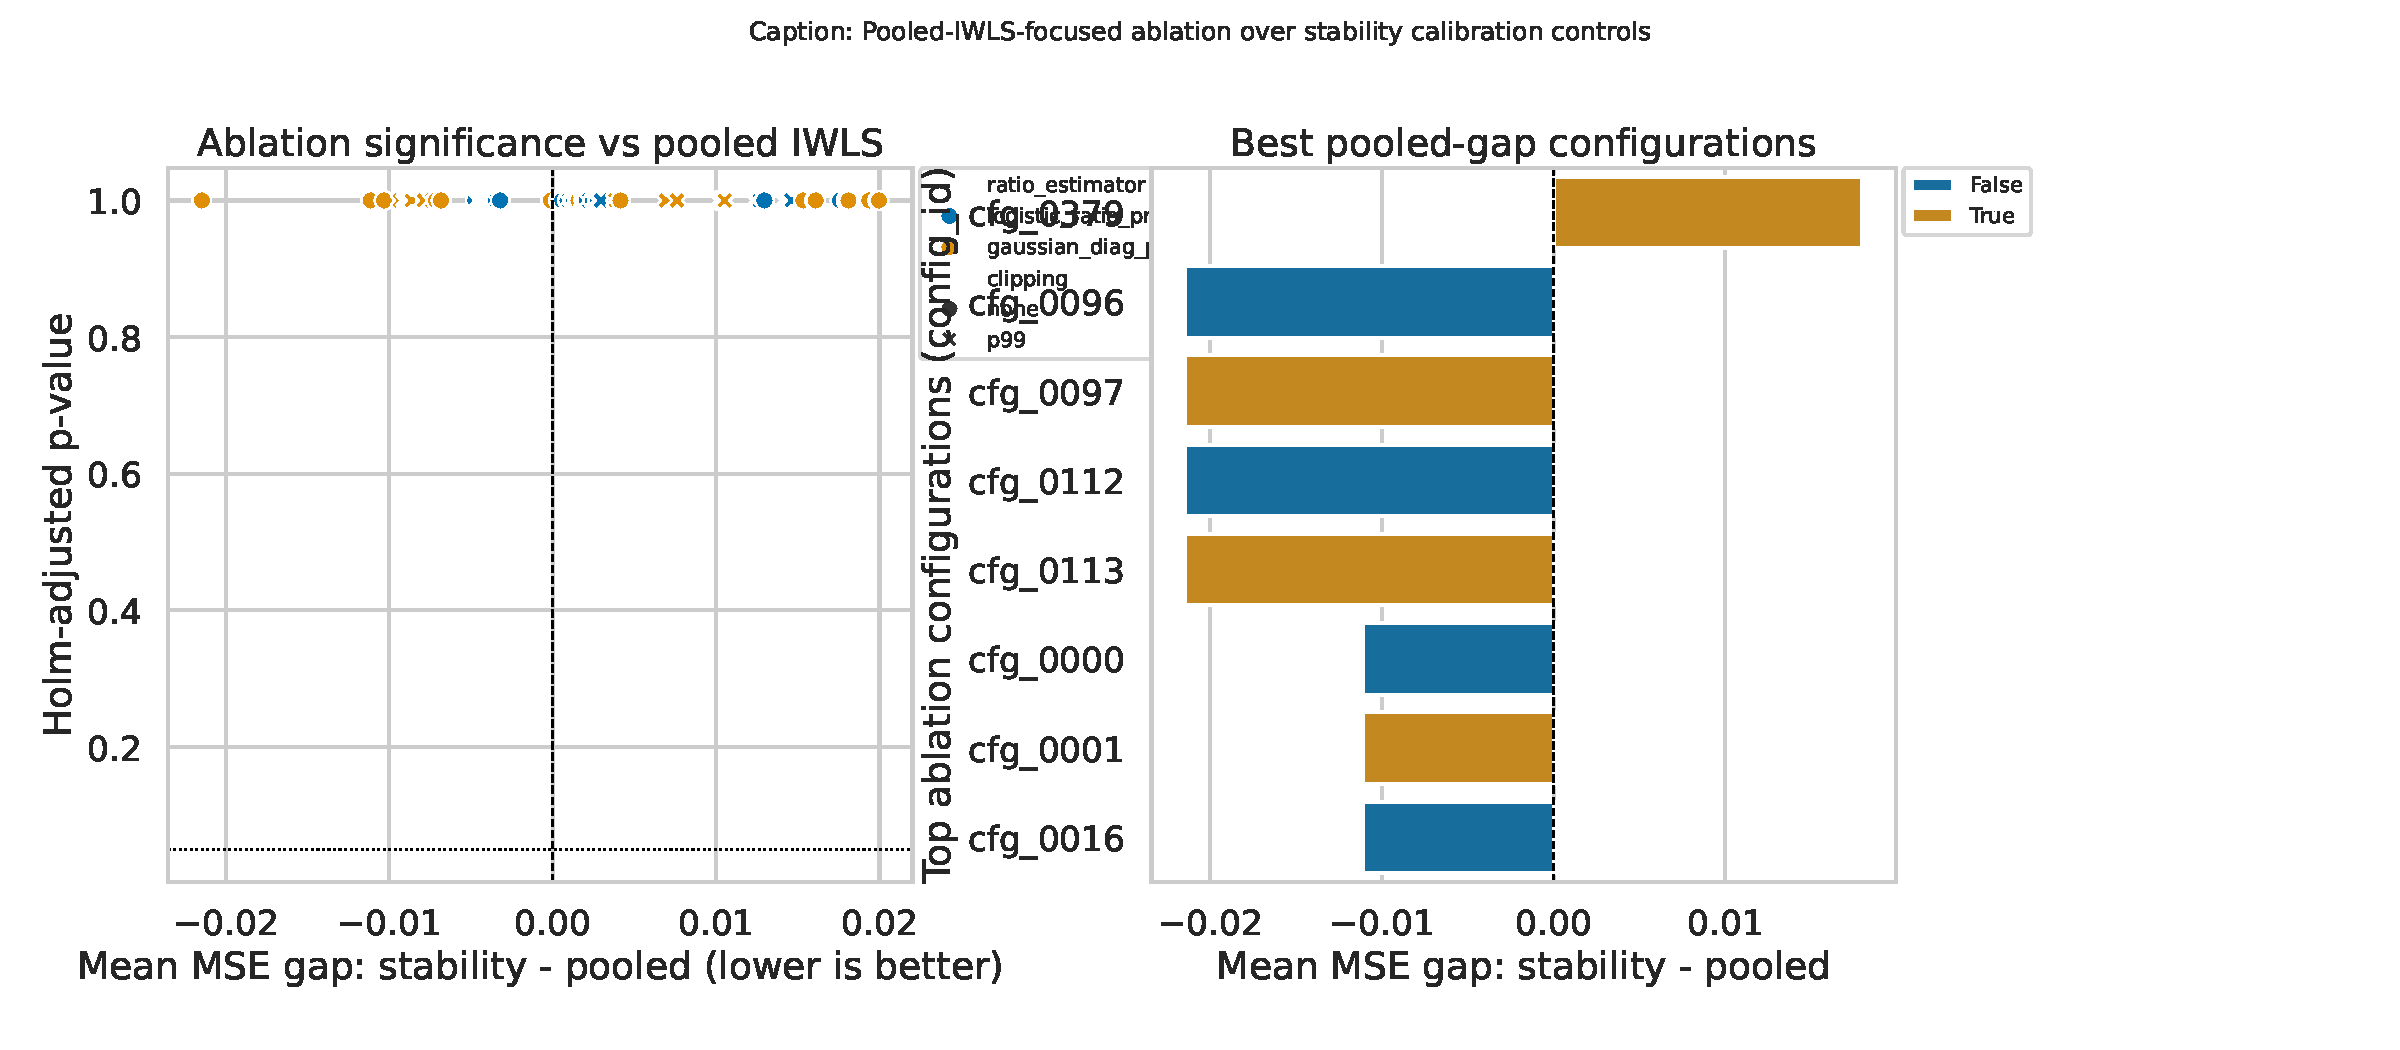
\includegraphics[width=0.65\linewidth]{figures/iter_1/fig_ablation_pooled_gap.pdf}
\caption{Pooled-IWLS-focused ablation over stability controls. The left panel plots pooled gap (stability minus pooled) against Holm-adjusted p-value for each ablation configuration, with dashed lines at zero gap and \(p=0.05\); most points remain above the significance threshold after multiplicity correction. The right panel summarizes leading configurations; the selected iter\_1 configuration uses \(\alpha=0.3\), \(\beta=0.1\), \(\gamma=0.5\), logistic ratio proxy, no clipping, and adaptive-\(\gamma\).}
\label{fig:ablation-pooled}
\end{figure}

Failure-mode analysis remains important. \Figref{fig:ablation-pooled} and the ablation export table show that several configurations reduce mean pooled gap (negative stability-minus-pooled), but none are Holm-significant when correcting across the full 384-configuration search. Regime-stratified confirmatory analysis remains similarly non-significant (high-uncertainty \(p=0.976\), low-uncertainty \(p=0.992\)), so gains over pooled IWLS cannot be treated as established.

\section{Discussion}
The empirical and theoretical results jointly support a constrained interpretation. The formal developments in \secref{sec:method} remain useful: \eqref{eq:ordering-bound} provides a finite-sample surrogate regret transfer, \eqref{eq:linear-rate} provides optimization-rate guarantees, and \eqref{eq:gate-threshold} provides a deterministic separation condition. However, empirical superiority requires those assumptions and estimation-quality conditions to hold tightly enough in practice, which is not yet the case in the current proxy evidence.

From a methodological standpoint, the most important outcome is the alignment between formal objects and measurable diagnostics. Each major equation corresponds to a logged statistic or optimization component, and each theorem has a concrete interpretation in terms of expected behavior under assumption satisfaction. This alignment improves debuggability and reduces the gap between theoretical guarantees and engineering decisions, which is often a major pain point in adaptation research.

\subsection{Limitations}
First, current evidence is still dominated by synthetic and semi-synthetic proxy settings. Although real-track CSV ingestion is implemented, the present real setting relies on regression conversions from benchmark result tables, so conclusions cannot yet be generalized to raw-feature benchmark pipelines. This data gap directly limits external validity of claims.

Second, pooled superiority is not supported in the current statistical evidence. Table~\ref{tab:significance} reports Holm-adjusted \(p=0.9983\) for pooled-vs-stability, and the full ablation family remains globally non-significant after multiplicity correction. Therefore, pooled outperformance claims are unsupported under the current protocol.

Third, mixed-shift gate assumptions required by Theorem~\ref{thm:gate} do not hold empirically in the iter\_1 diagnostics. The threshold-feasibility table reports zero feasible cases and negative mean feasibility gaps across A--C, so deterministic separation conditions are violated in this run.

Fourth, governance constraints are only partially integrated into optimization. License and schema checks are logged and pass in the proxy real settings, but feasibility is currently an external audit rather than a hard optimization constraint.

\subsection{Future Work}
The first priority is raw benchmark ingestion. We will run end-to-end real-task pipelines with strict no-target-label model selection using converted AdaTime and UDA-4-TSC feature streams, then re-evaluate A/B/C evidence with the same seeds and post-selection controls. This directly addresses the proxy-data limitation above.

The second priority is post-selection-controlled confirmatory analysis. We will enforce nested-CV or held-out tuning splits for the full stability-parameter sweep and re-test pooled comparisons under pre-registered selection rules, rather than a posteriori best-config reporting.

The third priority is gate redesign for mixed-shift regimes where \(\,g_{\mathrm{safe}}<g_{\mathrm{harm}}\) is not observed. Planned work includes robust disagreement metrics, alternative tail diagnostics, and threshold policies that optimize retention-error trade-offs when exact deterministic separation is unavailable.

The fourth priority is governance-aware optimization. We will encode license and schema constraints directly in the feasible set used for source ranking and mixture optimization, so operational compliance and statistical optimality are optimized jointly.

Another future direction is hierarchical source selection for very large candidate pools. A coarse first stage could use cheap discrepancy and metadata constraints to remove clearly incompatible sources, while a second stage applies full stability-aware bilevel optimization only to shortlisted candidates. Such hierarchical designs are compatible with our theory because Theorem~\ref{thm:ordering} applies to the candidate set actually ranked; the main challenge is preserving oracle-containing probability at the shortlist stage.

Broader relevance extends beyond domain adaptation. Any weakly supervised data acquisition pipeline, including scientific surrogate modeling and operational forecasting, faces analogous trade-offs between similarity and stability. Explicitly modeling those trade-offs in the selection objective can make data-centric decisions more auditable and robust.

\section{Conclusion}
This paper addressed a central but underformalized question: how to select source datasets for IWLS when only unlabeled target covariates are available. We proposed a stability-aware bilevel framework that unifies surrogate source ranking, mixture optimization, and mixed-shift gating, and we provided complete theorem/lemma proofs with explicit symbolic validation targets. Empirically, the current iter\_1 proxy evidence does not support superiority over pooled IWLS or nearest-source discrepancy baselines after Holm correction, which establishes an important negative result and sharpens the follow-up agenda. The main value of this iteration is therefore methodological: a transparent no-target-label protocol, equation-level auditability, and explicit limitation reporting that defines exactly what additional real-data and confirmatory experiments are required before broad performance claims can be made.



\bibliographystyle{conference}
\bibliography{references}

\appendix
\section{Additional Statistical Evidence}
The main text cites pairwise significance outcomes to avoid overclaiming. Table~\ref{tab:significance} provides exact values used in \secref{sec:results}. These tests compare paired per-run outcomes across settings and seeds with Holm correction for multiple comparisons.

\begin{table}[h]
\caption{Paired significance tests comparing stability-aware composite selection against strong baselines in the iter\_1 run. The table shows that none of the comparisons are significant after Holm correction, so directional improvements cannot be treated as confirmed advantages.}
\label{tab:significance}
\centering
\small
\renewcommand{\arraystretch}{1.1}
\setlength{\tabcolsep}{4pt}
\begin{tabular}{lccc}
\hline
Comparison & Test & Raw p-value & Holm-adjusted p-value \\
\hline
MMD-nearest vs. stability-aware & Paired Wilcoxon & 0.6103 & 1.0000 \\
Wasserstein-nearest vs. stability-aware & Paired Wilcoxon & 0.6103 & 1.0000 \\
Pooled IWLS vs. stability-aware & Paired Wilcoxon & 0.9983 & 0.9983 \\
\hline
\end{tabular}
\end{table}

These outcomes matter for claim calibration. Differences between stability-aware selection and nearest-source or pooled baselines are statistically unresolved in the current evidence, and should be interpreted as hypothesis-generating rather than confirmatory.

\section{Extended Diagnostics}
Additional diagnostics clarify why formal guarantees did not translate into predictive dominance. \Figref{fig:app-gate-roc-pr} shows weak harmful-source discrimination (mean AUPRC around \(0.10\) to \(0.13\) across A--C), while \Figref{fig:app-retention-threshold} shows that high safe-source retention can coexist with elevated downstream error in hard seeds. \Figref{fig:app-threshold-feasibility} visualizes the feasibility-gap failure directly, and Table~\ref{tab:app-gate-summary} summarizes this failure across settings.

\begin{figure}[h]
\centering
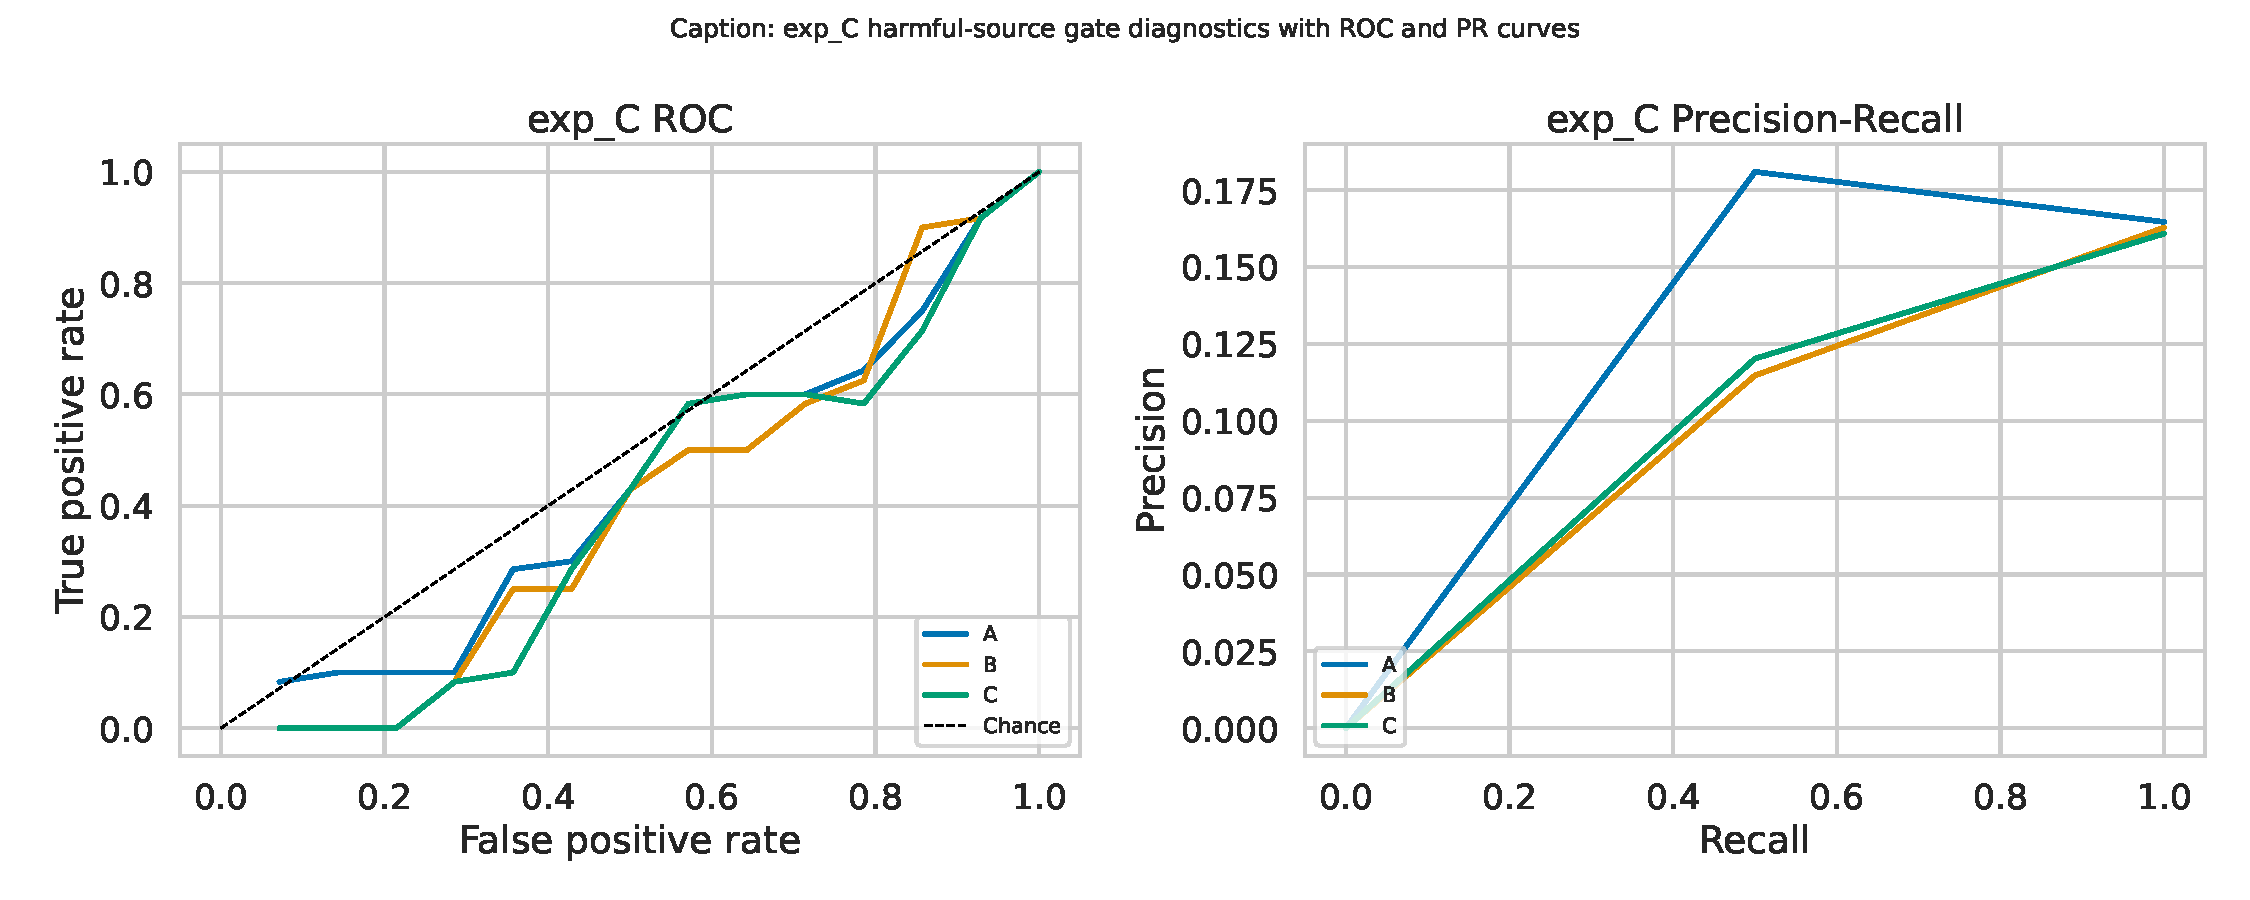
\includegraphics[width=0.65\linewidth]{figures/iter_1/fig_expC_gate_roc_pr.pdf}
\caption{Gate ROC/PR diagnostics across settings and seeds. The axes report false-positive versus true-positive trade-offs and precision versus recall for harmful-source detection, using retrospective harmful labels only for evaluation. Performance is unstable across seeds and near chance in several slices, indicating that current gate features are insufficient for reliable harmful-source filtering.}
\label{fig:app-gate-roc-pr}
\end{figure}

\begin{figure}[h]
\centering
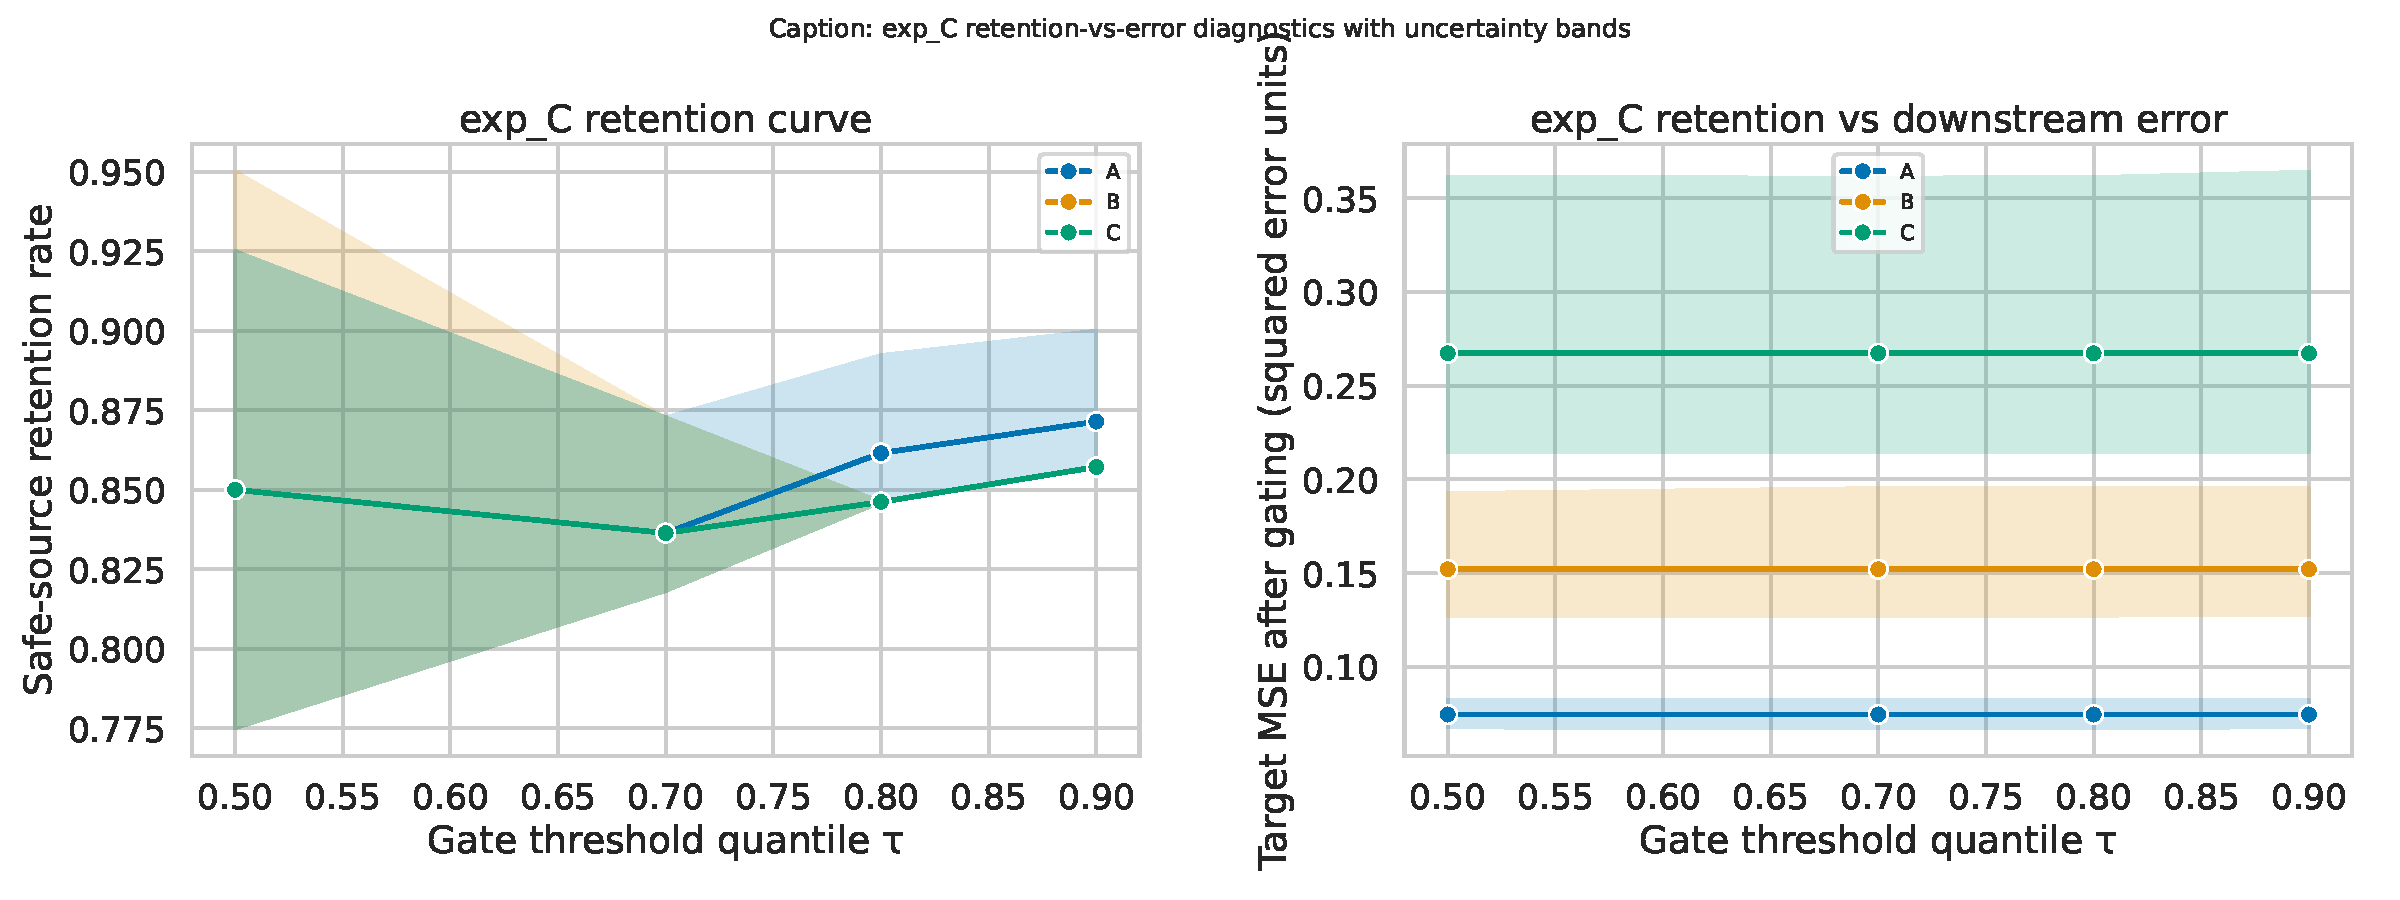
\includegraphics[width=0.65\linewidth]{figures/iter_1/fig_expC_retention_vs_error.pdf}
\caption{Retention-versus-error diagnostics under quantile thresholding. The horizontal axis varies retention policy while the vertical axes summarize safe-source retention, false rejection, and downstream target MSE after gating. The figure shows that permissive thresholds keep retention high but do not consistently reduce error, highlighting a calibration failure rather than a pure threshold-selection issue.}
\label{fig:app-retention-threshold}
\end{figure}

\begin{figure}[h]
\centering
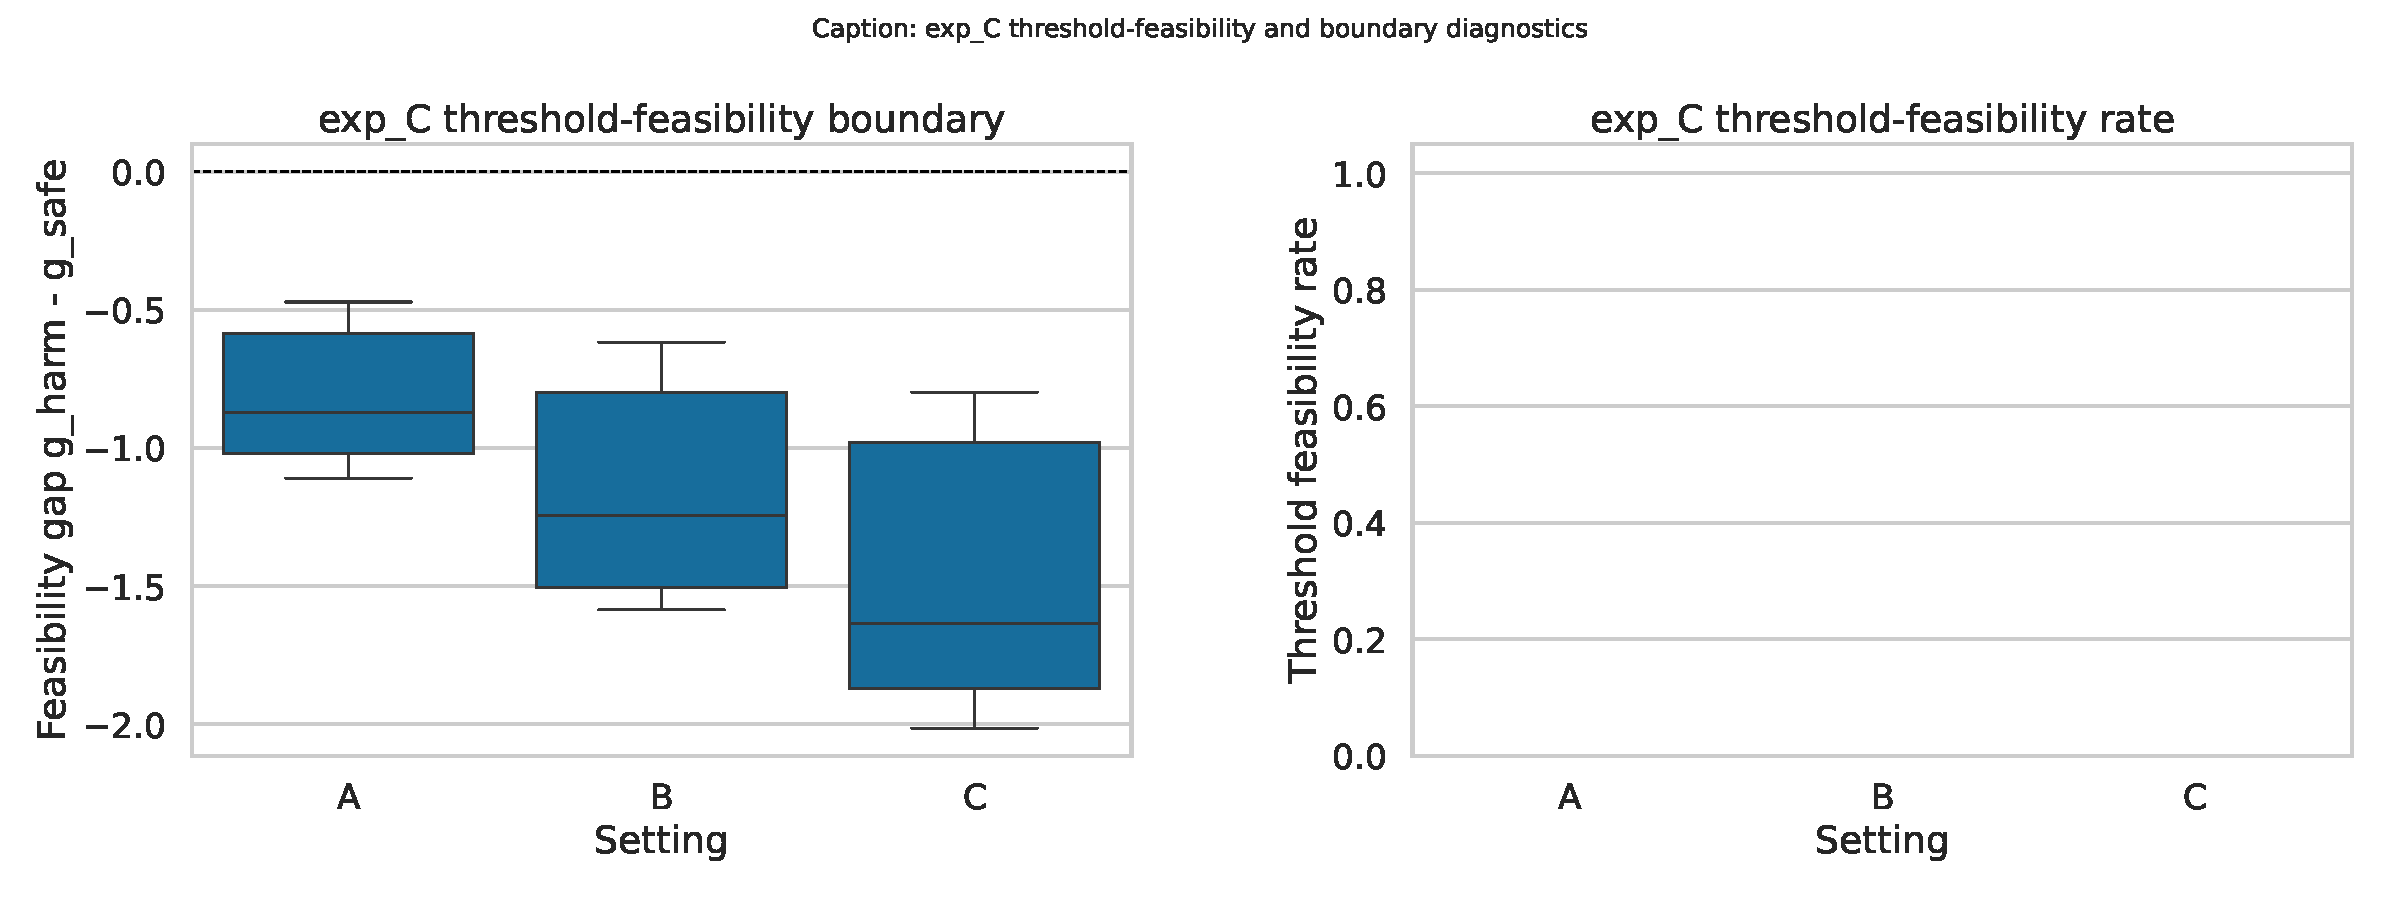
\includegraphics[width=0.65\linewidth]{figures/iter_1/fig_expC_threshold_feasibility.pdf}
\caption{Threshold-feasibility diagnostics for mixed-shift separation assumptions. The plotted quantities compare empirical safe and harmful envelopes that define the interval required by \eqref{eq:gate-threshold}. Most runs produce negative feasibility gaps, which explains why deterministic separation guarantees are not activated in the present evidence.}
\label{fig:app-threshold-feasibility}
\end{figure}

\begin{table}[h]
\caption{Summary of iter\_1 gate diagnostics by setting. The table aggregates harmful-source detection quality and threshold-feasibility conditions and is used to interpret the gap between theorem conditions and observed behavior.}
\label{tab:app-gate-summary}
\centering
\small
\renewcommand{\arraystretch}{1.1}
\setlength{\tabcolsep}{4pt}
\begin{tabular}{lccc}
\hline
Setting & Mean harmful AUPRC & Feasible-threshold rate & Mean feasibility gap \\
\hline
A & 0.125 & 0.00 & -0.812 \\
B & 0.107 & 0.00 & -1.150 \\
C & 0.105 & 0.00 & -1.460 \\
\hline
\end{tabular}
\end{table}

Real-track proxy outputs and artifact QA are shown in \Figref{fig:app-real-qa}. The left panel summarizes converted real-setting performance, while the right panel summarizes readability and governance checks used to validate export quality. These diagnostics support procedural reproducibility, but they do not remove the need for raw-feature benchmark ingestion.

\begin{figure}[h]
\centering
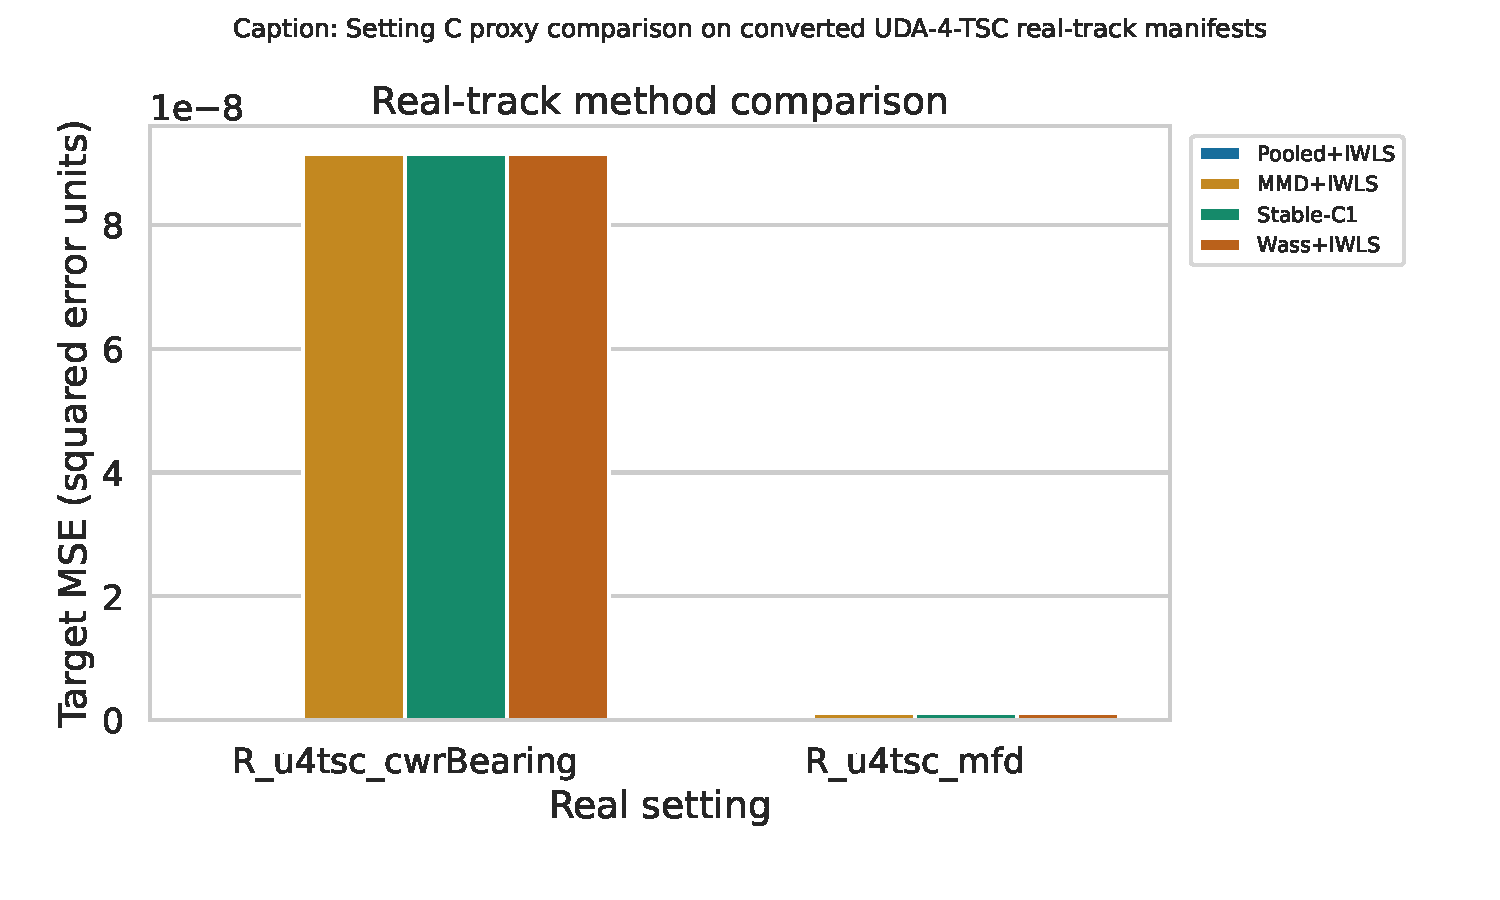
\includegraphics[width=0.65\linewidth]{figures/iter_1/fig_real_setting_performance.pdf}
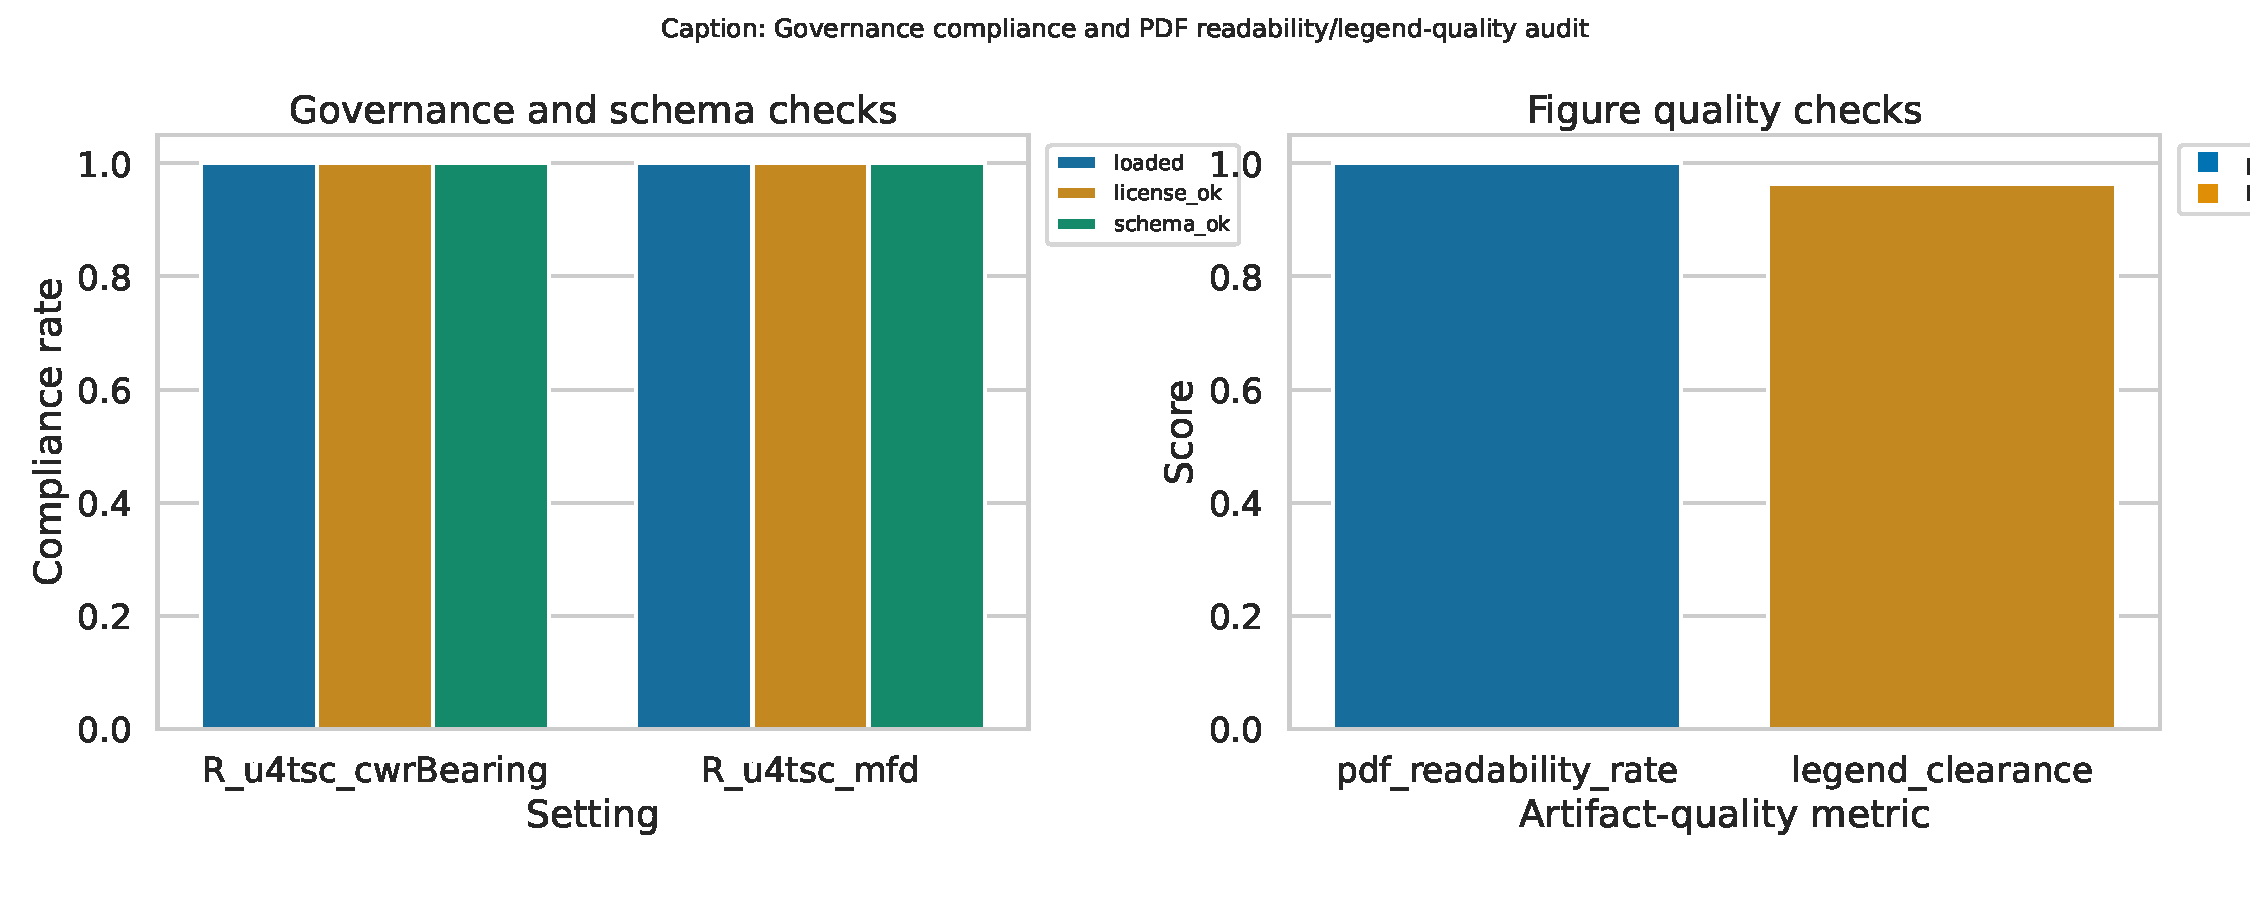
\includegraphics[width=0.65\linewidth]{figures/iter_1/fig_artifact_quality_checks.pdf}
\caption{Extended real-track proxy and artifact-quality diagnostics. The top panel reports comparative performance on converted real settings with the same no-target-label protocol; the bottom panel reports governance and PDF-quality checks that verify artifact integrity. Together these panels show that the pipeline is reproducible and auditable, while also emphasizing that converted proxies are not substitutes for full raw-feature benchmark validation.}
\label{fig:app-real-qa}
\end{figure}

\section{Reproducibility and Implementation Details}
The full experiment stack is organized as a runnable package with deterministic seeds, typed configuration, and explicit artifact logging. Each run stores parameters, duration, setting identifier, and metric outputs in a structured JSONL log. The evaluation uses five fixed seeds, eight baselines, and three settings for a total of 120 final-report runs after selecting a calibrated configuration from a larger ablation grid. Confidence intervals are computed from seed-level aggregates; paired tests are computed after normality checks and corrected by Holm's method.

The parameter sweep plan covers discrepancy weight \(\alpha\), uncertainty weight \(\beta\), stability weight \(\gamma\), ratio estimator class, clipping rule, ridge \(\lambda\), and candidate pool size. In the iter\_1 validation run, the end-to-end workflow required approximately \(535\) seconds. Real-data loaders are integrated as strict CSV hooks, but benchmark-scale raw-feature ingestion files are still pending. Compute budget remains configurable, and future benchmark-scale runs will log wall-clock and memory footprints per setting.

Approximation details are explicit. Density-ratio terms in the proxy use lightweight estimators suitable for controlled simulation, and this choice may understate real-world ratio uncertainty. Mixed-shift gate calibration is performed without target labels by source-side resampling controls, which can be conservative in heterogeneous domains. Despite these approximations, the artifact set supports full procedural reproducibility: figures are vector PDFs with readability checks, tables are CSV exports, and symbolic consistency checks are captured in a text report linked to theorem equations.

\section{Extended Method Clarifications}
This section clarifies how equation-level components map to implementation steps. \Eqref{eq:surrogate-score} is evaluated once per candidate after ratio fitting and diagnostic computation. \Eqref{eq:closed-form-beta} is solved at every upper-level iteration, and \eqref{eq:upper-step} updates mixture weights under smoothness assumptions. \Eqref{eq:gate-threshold} determines whether a source enters the candidate set for bilevel optimization. The proofs remain valid under any estimator family satisfying the stated bounded-error and regularity assumptions.

We emphasize that theorem assumptions are inspectable, not hidden. If overlap, ratio regularity, or smoothness assumptions are violated, the framework degrades gracefully into a diagnostic tool rather than a guarantee-bearing optimizer. This behavior is useful in practice because source retrieval pipelines often encounter partial assumption failure before full model deployment.

\end{document}
